\section{Projektmonitoring}
\label{sec:Projektmonitoring}

\subsection{Auswertung Velocity}
\label{sub:Auswertung Velocity}

\begin{figure}[H]
    \centering
    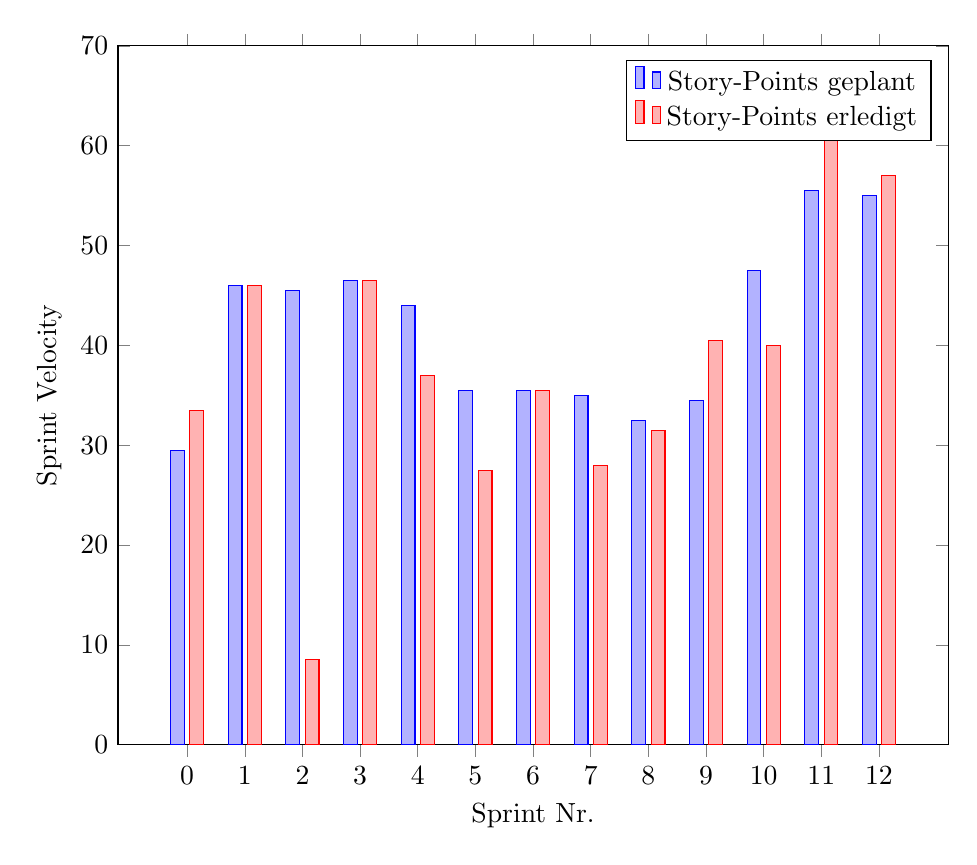
\begin{tikzpicture}
        \begin{axis}[
            ybar,
            width=1\textwidth,
            bar width=5pt,
            ylabel={Sprint Velocity},
            xlabel={Sprint Nr.},
            ymin=0,
            ymax=70,
            xtick=data,
            % nodes near coords,
            % nodes near coords align={vertical},
            % every node near coord/.append style={color=black, font=\tiny}
        ]
            \addplot[style={blue, fill=blue!30!white}] coordinates
                {(0, 29.5) (1, 46) (2, 45.5) (3, 46.5) (4, 44) (5, 35.5) (6, 35.5) (7, 35)
                (8, 32.5) (9, 34.5) (10, 47.5) (11, 55.5) (12, 55)};
            \addplot [style={red, fill=red!30!white}] coordinates
                {(0, 33.5) (1, 46) (2, 8.5) (3, 46.5) (4, 37) (5, 27.5) (6, 35.5) (7, 28)
                (8, 31.5) (9, 40.5) (10, 40) (11, 60.5) (12, 57)};
            \legend{Story-Points geplant,Story-Points erledigt}
        \end{axis}
    \end{tikzpicture}%

    \caption[Diagramm Velocity über das Projekt]{Sprint Velocity über den Verlauf des Projekts}
    \label{chart:sprint_velocity}
\end{figure}

In Abbildung \ref{chart:sprint_velocity} ist die Velocity für jeden Sprint über den Verlaufs des Projekts aufgezeichnet. Die Velocity besteht jeweils aus der Anzahl der geplanten und effektiv durchgeführten Story-Points. Jeder Sprint dauerte eine Woche.

Im Diagramm \ref{chart:sprint_velocity} ist auffällig, dass wir zu Beginn gerade eine hohe Velocity erreichten, die in Sprint 2 dann völlig einbrach. Dies lag hauptsächlich an zu grossen Arbeitspaketen, die kaum in einem Sprint erledigt werden konnten. Mit dieser Erkenntnis haben wir die weiteren Arbeitspakete aufgeteilt und im Sprint 3 wieder mit der Velocity von Sprint 2 geplant. Dies hat auch funktioniert, gegen Mitte des Projektes sinkte sie allerdings wieder auf ca. 35 und pendelte sich dort ein. Durch den Zeitdruck gegen Ende des Projektes stieg die Velocity wieder, damit wir die offenen Arbeitspakete noch vor dem Abgabetermin erledigen konnten.


\subsection{Zeitauswertung}
\label{sub:Zeitauswertung}

\begin{figure}[H]
    \centering
    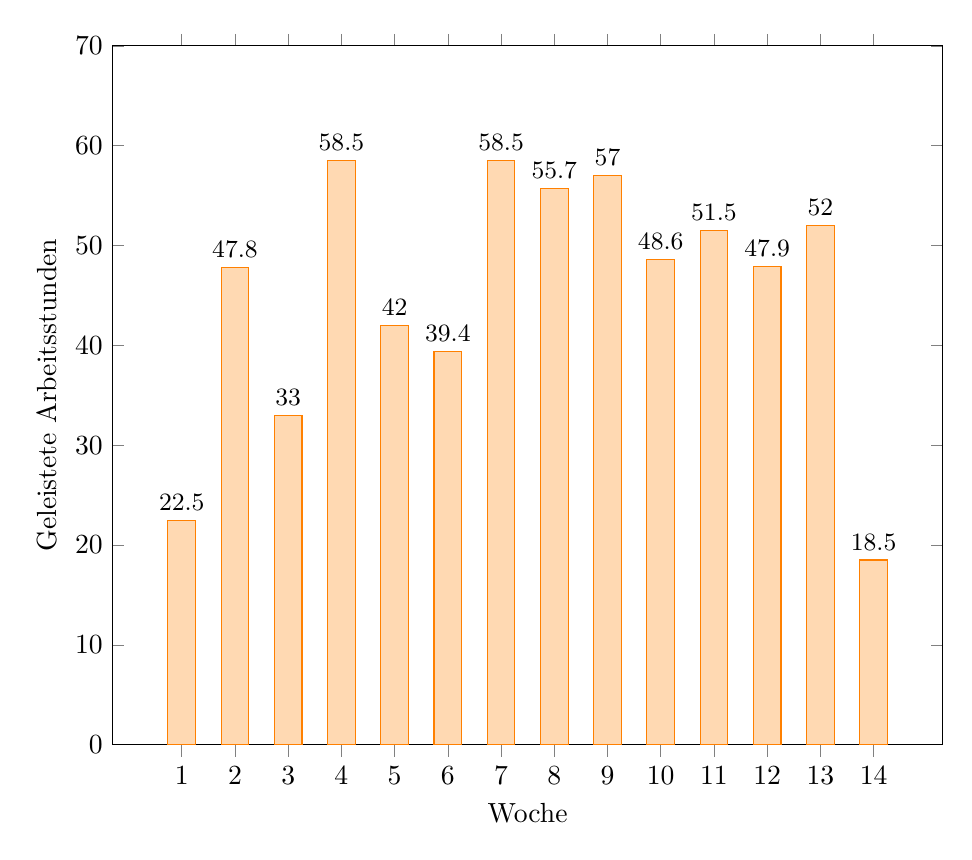
\begin{tikzpicture}
        \begin{axis}[
            ybar,
            width=1\textwidth,
            bar width=10pt,
            ylabel={Geleistete Arbeitsstunden},
            xlabel={Woche},
            ymin=0,
            ymax=70,
            xtick=data,
            nodes near coords,
            nodes near coords align={vertical},
            every node near coord/.append style={color=black, font=\small}
        ]
            \addplot[style={orange, fill=orange!30!white}] coordinates
                {(1, 22.5) (2, 47.8) (3, 33) (4, 58.5) (5, 42) (6, 39.4) (7, 58.5)
                (8, 55.7) (9, 57) (10, 48.6) (11, 51.5) (12, 47.9) (13, 52) (14, 18.5)};
        \end{axis}
    \end{tikzpicture}

    \caption[Diagramm Zeitaufwand über den Verlauf des Projekts]{Zeitaufwand über den Verlauf des Projekts (Stand 19.12.2017)}
    \label{chart:Zeitauswertung}
\end{figure}

In Abbildung \ref{chart:Zeitauswertung} ist aufgezeigt, wie viele Stunden pro Woche über den Verlauf des Projekts geleistet wurden. Das gesamte Zeitbudget betrug dabei \textbf{480} Stunden, was pro Woche ca. 34 Stunden entspricht.

Die total geleisteten Arbeitsstunden im Team sind mit \textbf{328h} (Jonas Matter) und \textbf{310h} (Robin Suter) ähnlich verteilt (Stand 19.12.2017).

Wie man in Abbildung \ref{chart:Zeitauswertung} sieht, ist die geleistete Zeit pro Woche ausser zu Beginn jeweils über dem eingeplanten Zeitbudget. Dies liegt wohl daran, dass wir um die Woche 4 eine hohe Velocity erreichten (siehe \ref{sub:Auswertung Velocity}), dafür aber viel Zeit investierten. In den nachfolgenden Wochen behielten wir die Velocity ungefähr bei, der Zeitaufwand blieb aber gleich hoch. Schlussendlich führte dies dazu, dass wir alle Projektziele erreichen konnten, dafür aber deutlich mehr Arbeitsaufwand als geplant investiert haben.

\subsection{Codestatistik}
\label{sub:Codestatistik}

In Tabelle \ref{table:Code-Metriken} sind einige Code-Metriken aufgelistet. Diese sind natürlich mit Vorsicht zu geniessen, da diese nur bedingt etwas über die Softwarequalität aussagen können. Es ist aber gut zu sehen, welchen Umfang die einzelnen Komponenten im Verhältnis zum Gesamtsystem ausmachen.

\begin{table}[ht]
    \centering
    \caption{Code-Metriken}
    \label{table:Code-Metriken}
    \begin{tabular}{p{10cm}r}
        \toprule
        \textbf{Anzahl Zeilen Produktiv-Code}           & \textbf{2328} \\
            \hspace{1em} \code{plaza\_preprocessing}    & 969           \\
            \hspace{1em} \code{plaza\_routing}          & 723           \\
            \hspace{1em} QGIS-Plugin                    & 636           \\
        \midrule
        \textbf{Anzahl Tests}                           & \textbf{74}   \\
            \hspace{1em} \code{plaza\_preprocessing}    & 29            \\
            \hspace{1em} \code{plaza\_routing}          & 45            \\
        \midrule
        \textbf{Test Coverage}                          & \textbf{83\%}   \\
            \hspace{1em} \code{plaza\_preprocessing}    & 88\%          \\
            \hspace{1em} \code{plaza\_routing}          & 78\%          \\
    \end{tabular}
\end{table}